\documentclass[a4paper]{article}
\usepackage[utf8]{inputenc}
\usepackage[russian,english]{babel}
\usepackage[T2A]{fontenc}
\usepackage[left=10mm, top=20mm, right=18mm, bottom=15mm, footskip=10mm]{geometry}
\usepackage{indentfirst}
\usepackage{amsmath,amssymb}
\usepackage[italicdiff]{physics}
\usepackage{graphicx}
\graphicspath{{images/}}
\DeclareGraphicsExtensions{.pdf,.png,.jpg}
\usepackage{wrapfig}

\usepackage{caption}
\captionsetup[figure]{name=Рисунок}
\captionsetup[table]{name=Таблица}
  
\title{\underline{Отчет о выполненой лабораторной работе 1.4.2}}
\author{Антон Хмельницкий, Б01-306}


\begin{document}

\maketitle
\textbf{Изучение экспериментальных погрешностей на примере физического маятника}

\section{Аннотация}
\underline{Цель работы}: 
\begin{enumerate}
    \item На примере измерения периода свободных колебаний физического маятника познакомиться систематическими и случайными погрешностями, прямыми и косвенными измерениями; 
    \item Проверить справедливость формулы для периода колебаний физического маятника и определить значение ускорения свободного падения; 
    \item Убедиться в справедливости теоремы Гюйгенса об обратимости точек опоры и центра качания маятника; 
    \item Оценить погрешность прямых и косвенных измерений и конечного результата.
\end{enumerate} \par
\underline{Оборудование}: металлический стержень с опорной призмой; дополнительный груз; закреплённая на стене консоль; подставка с острой гранью для определения цента масс маятника; электронный секундомер; электронный счётчик колебаний; линейки металлические различной длины; штангенциркуль; электронные весы;

\section{Теоретические сведения}

Физическим маятником называют твёрдое тело, способное совершать колебания в вертикальной плоскости, будучи подвешено за одну из своих точек в поле тяжести. Основное отличие физического маятника от математического в том, что маятник не является точечным объектом, а представляет собой совокупность жёстко связанных точечных масс. В данной работе в качестве такого маятника

\subsection{Момент инерции для стержня}
Для динамики движения точечной массы m под действием
силы F вдоль некоторой прямой справедливо уравнение Ньютона:
\[F = \frac{dp}{dt},\text{  где $p = mv$ - импульс, $v$ - скорость тела.}\]
При вращательном движении момент относительно оси вращения $M = Fr$, тогда уравнение Ньютона преобразуем:
\[Fr = \frac{d(m(\omega r) \cdot r)}{dt} \longrightarrow M = \frac{dL}{dt}, \text{ где $L = m\omega r^2$}\]
Вводится обозначение $J = m r^2$ - момент инерции точечного тела. $ L = J\omega$ - момент импльса(вращательный импульс). Получаем уравнение:
\[M = J\frac{d\omega}{dt}\]
В случае твердого тела состоящего из совокупности материальных точек, вращающихся вокруг одной оси момент импульса вычисляется как:
\[J = \sum\limits_{i}^{N} m_{i}r_{i}^2, \text{ где $r_{i}$ - расстояние от $m_{i}$ точки до оси вращения}\]
Из курса механики момент инерции тонкого стержня массой $m$ и длиной $l$, вращающегося вокруг оси, проходящей через центр масс, равен:
\[J_{c} = \frac{ml^2}{12}\]
А момент инерции стержня, подвешенного на расстоянии $a$ от центра масс, может быть вычислен по теореме Гюйгенса–Штейнера: 
\[J = \frac{ml^2}{12} + ma^2\]

\subsection{Общая формула физического маятника}

\begin{wrapfigure}{R}{.3\textwidth}
\centering
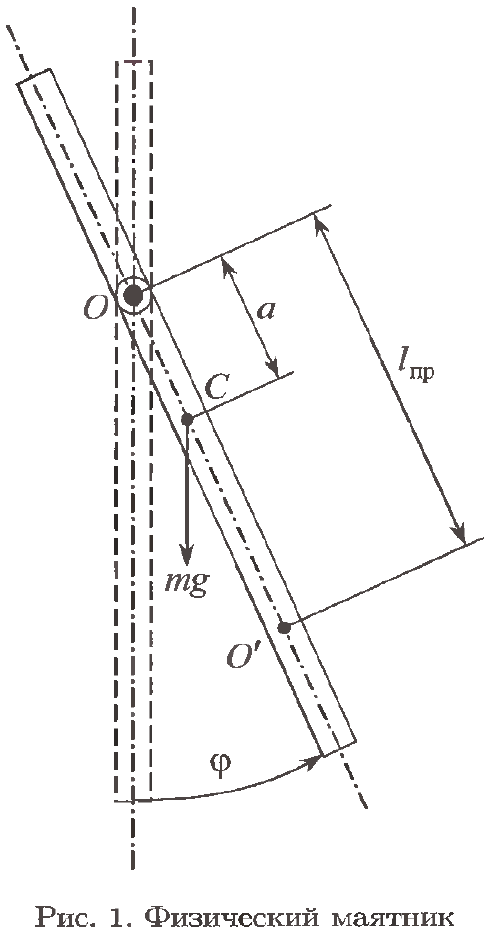
\includegraphics[width=.25\textwidth]{shema.png}
\caption{Схема включения счетчика}
\end{wrapfigure}

Маятник подвешен в точке $O$ на расстоянии $a$ до центра масс $C$ (рис.1).

Общая формула для периода колебаний произвольного физического маятника:
\[T = 2\pi \sqrt{\frac{J}{mga}}\]
А для стержня длиной $l$, подвешенного на расстоянии $a$ от центра, получаем:
\[T = 2\pi \sqrt{\frac{\frac{l^2}{12}+a^2}{ga}}\]
Для математического маятника будет:
\[T = 2\pi \sqrt{\frac{l}{g}}\]
Определим так называемую приведённую длину физического маятника.Смысл этой длины в том, что физический маятник длиной $l$, подвешенный в точке $a$, имеет тот же период малых колебаний, что и математический маятник длиной $l_{\text{пр}}$:
\[l_{\text{пр}} = a + \frac{l^2}{12a}\]
\underline{Теорема Гюйгенса}: Рассмотрим точку $O^{'}$, отстоящую от точки опоры $O$ на расстояние $l_{\text{пр}}$ вдоль стержня (эту точку иногда
называют центром качания физического маятника). Оказывается, если маятник подвесить за точку $O^{'}$, то период его качания не изменится. Иными словами, точка опоры и центр качания маятника взаимно обратимы.

\subsection{Затухающие колебания}
Амплитуду колебаний следует считать медленно убывающей функцией времени: $A(t)$.

Относительную убыль амплитуды за одно колебание $\gamma = |\frac{\delta A}{A}|$ называют декрементом затухания.

Получаем экспненциальную зависимость амплитуды колебаний от времени:
\[A(t) = A_{0} \cdot e^{-\gamma t}\]
Таким образом, величина $\tau_{k} = \frac{1}{\gamma}$ — это время, за которое амплитуда колебаний падает в $e$ раз.

В теории колебаний принято использовать безразмерную характеристику затухания, называемую добротностью колебательной системы:
\[Q = \pi\frac{\tau_{k}}{T}\]

\subsection{Погрешность при измерении периода колебаний}
В работе использовался электронный секундомер и электронный счетчик, поэтому $\sigma_{t}^{\text{сист}} = 0,01$с определяется по последнему разряду прибора.

Случайную погрешность вычислим по формуле среднеквадратического отклонения:
\[\sigma_{t}^{\text{случ}} = \sqrt{\frac{1}{n-1}\sum\limits_{i=1}^{n} (t_{i} - \overline{t})^2} = 0,0006\]
Полная погрешность:
\[\sigma_{t}^{\text{полн}} = \sqrt{(\sigma_{t}^{\text{сист}})^2 + (\sigma_{t}^{\text{случ}})^2} = 0,01002 \approx 0,01\]

Из измеренных данных получаем $\overline{T} \approx 1,526, \sigma_{t}^{\text{полн}} = 0,01,  \sigma_{T} = \frac{\sigma_{t}}{n}$ и $\varepsilon_{T} = \frac{\sigma_{T}}{T} < 10^{-3} (0,1\%)$ условие точности. Получаем:
\[n > \frac{\sigma_{t}}{\overline{T} \varepsilon_{T}} \approx 6,55 \longrightarrow n = 7 \text{ - достаточно для точности меньше 0,1\%}\]



\begin{table}[!h]
\begin{center}
\begin{tabular}{|l|l|l|l|}
\hline
№ опыта & Полное время t & Число колебаний n & Период T=t/n \\ \hline
1       & 30,53          & 20                & 1,5265       \\ \hline
2       & 30,55          & 20                & 1,5275       \\ \hline
3       & 30,52          & 20                & 1,526        \\ \hline
4       & 30,54          & 20                & 1,527        \\ \hline
\end{tabular}
\caption{Данные для определения достаточного n числа колебаний для минимальной погрешности}
\end{center}
\end{table}

\subsection{Особенности маятника с перемещаемым грузом}

\begin{wrapfigure}{R}{.3\textwidth}
\centering
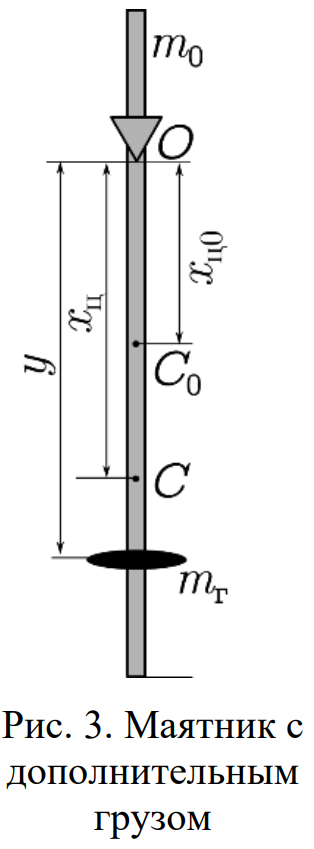
\includegraphics[width=.2\textwidth]{shema2.png}
\caption{Схема включения счетчика}
\end{wrapfigure}

Если на стержень насадить груз, то момент инерции маятника, а значит и период его колебаний, будет зависеть от положения груза относительно
оси качания. В качестве подвижного груза в работе используется металлический цилиндр или «чечевица».

Поскольку размер груза мал по сравнению с длиной стержня, его можно
считать закреплённой на стержне точечной массой. Обозначим за y расстояние от точки подвеса O до центра масс груза. Тогда момент
инерции маятника будет равен:
\[J = J_{0} + m_{\text{г}}y^2 = \frac{m_{0}l^2}{12} + m_{0}a^2 + m_{\text{г}}y^2\text{, ($m_{0} = m_{\text{ст}}$)}\]

Пусть $x_{\text{ц0}}$ — расстояние от точки подвеса (острия
призмы) до центра масс маятника без груза. Тогда центр
масс маятника с грузом $x_{\text{ц}}$ находится в точке:
\[x_{\text{ц}} = \frac{m_{0}x_{\text{ц0}} + m_{\text{г}}y}{M}\text{, где $M = m_{0} + m_{\text{г}}$ - полная масса маятника}\]
Отсюда $y$ будет равен:
\[y = \frac{M x_{\text{ц}} - m_{0}x_{\text{ц0}}}{m_{\text{г}}}\]
Из обще формулы периода колебаний:
\[T = 2\pi \sqrt{\frac{J_{0} + m_{\text{г}}y^2}{gM x_{\text{ц}}}} = 2\pi \sqrt{\frac{\frac{m_{0}l^2}{12} + m_{0}a^2 + m_{\text{г}}y^2}{gM x_{\text{ц}}}}\]

\subsection{Поправка для призмы}
В предыдущем пункте не было учета, что точка опоры - призма не материальная точка, поэтому сама имеет момент инерции, тогда для поправки преобразуем формулы для центра масс и соответственно:
\[x_{\text{ц}} = \frac{m_{0}x_{\text{ц0}} + m_{\text{г}}y}{M} = \frac{(m_{\text{ст}} + m_{\text{пр}})x_{\text{ц0}} + m_{\text{г}}y}{m_{\text{ст}} + m_{\text{пр}} + m_{\text{г}}},\]
где $x_{\text{ц0}}$ - центр массы "призма + стержень" и $M = m_{0} + m_{\text{ст}} + m_{\text{пр}}$ 
\newline 
\newline 
Заметим, что призма назодится близко к оси вращения, поэтому $J_{\text{пр}}$ не будет влиять на погрешность в том же порядке как наличие у призмы массы $m_{\text{пр}}$, поэтому в итоге получаем:
\[y = \frac{M x_{\text{ц}} - m_{0}x_{\text{ц0}}}{m_{\text{г}}} = \frac{M x_{\text{ц}} - (m_{\text{ст}} + m_{\text{пр}})x_{\text{ц0}}}{m_{\text{г}}}\]
\[T = 2\pi \sqrt{\frac{\frac{(m_{\text{ст}} + m_{\text{пр}})l^2}{12} + (m_{\text{ст}} + m_{\text{пр}})a^2 + m_{\text{г}}y^2}{g (m_{\text{ст}} + m_{\text{пр}} + m_{\text{гр}}) x_{\text{ц}}}}\]
\[T = 2\pi \sqrt{\frac{\frac{(m_{\text{ст}} + m_{\text{пр}})l^2}{12} + (m_{\text{ст}} + m_{\text{пр}})a^2 + m_{\text{г}}y^2}{g ((m_{\text{ст}} + m_{\text{пр}})a + m_{\text{г}}y)}}\]
\[T = 2\pi \sqrt{\frac{\frac{(m_{\text{ст}} + m_{\text{пр}})l^2}{m_{\text{г}}12} + \frac{(m_{\text{ст}} + m_{\text{пр}})}{m_{\text{г}}}a^2 + y^2}{g \left( \frac{(m_{\text{ст}} + m_{\text{пр}})}{m_{\text{г}}}a + y \right) }}\]

Пусть $\beta = \frac{m_{\text{пр}} + m_{\text{ст}}}{m_{\text{г}}} \approx 3,02 \pm 0,0005$, тогда $T$ будет равен:
\[T = 2\pi \sqrt{\frac{\frac{\beta l^2}{12} + \beta a^2 + y^2}{g \left( \beta a + y \right)}}\]

Тогда наиболее точная формула вычисления $g(T)$ будет:
\[g = \frac{4\pi^2(\frac{(m_{\text{ст}} + m_{\text{пр}})l^2}{12} + (m_{\text{ст}} + m_{\text{пр}})a^2 + m_{\text{г}}y^2)}{T^2 (m_{\text{г}} + m_{\text{ст}} + m_{\text{пр}}) x_{\text{ц}}}\]
\[g = \frac{4\pi^2(\frac{\beta l^2}{12} + \beta a^2 + y^2)}{T^2 (1 + \beta) x_{\text{ц}}}\]
Отсюда видно, что если построить зависимость величины $u = T^2 x_{\text{ц}}$  от $v = y^2$, то график должен иметь вид прямой линии. По её наклону можно определить ускорение свободного падения $g$, а по вертикальному смещению — момент инерции $J_{0}$ маятника.
\newpage
\section{Характеристики приборов и их погрешности}


\begin{table}[!h]
\begin{center}
\begin{tabular}{|l|l|l|}
\hline
Длина стержня, $l$                              & 100,1 см & Погрешность штангенциркуля 0,1 мм    \\ \hline
Центр масс пустого стержня, $x_{\text{ст}}$                 & 50,2 см  & Погрешность линейки 0,5 мм           \\ \hline
Центр массы "призмы + стержень" отн. О, $a = x_{\text{ц0}}$ & 27,4 см  & Погрешность линейки 0,5 мм           \\ \hline
Масса стержня, $m_{\text{ст}}$            & 868,2 г  & Погрешность весов по паспорту 0,5 г  \\ \hline
Масса доп груза, $m_{\text{гр}}$          & 314 г    & Погрешность весов по паспорту 0,5 г \\ \hline
Масса призмы, $m_{\text{пр}}$             & 79,6 г   & Погрешность весов по паспорту 0,5 г \\ \hline
Достаточное число колебаний, $n$ & 7 & Погрешность < 0,1\% по выкладке выше \\ \hline 
\end{tabular}
\caption{Данные для определения достаточного n числа колебаний для минимальной погрешности}
\end{center}
\end{table}


\section{Расчет данных}
\subsection{Полученные данные}
\begin{table}[!h]
\begin{center}
\begin{tabular}{|l|l|l|}
\hline
Центр масс   системы, $x_{\text{ц}}$, см & Время колебаний, $t$, с & Число колебаний,  $n$ \\ \hline
37,4                                      & 11,05                 & 7                     \\ \hline
35,8                                      & 10,8                  & 7                     \\ \hline
34,9                                      & 10,68                 & 7                     \\ \hline
33,5                                      & 10,47                 & 7                     \\ \hline
32,8                                      & 10,37                 & 7                     \\ \hline
32,2                                      & 10,29                 & 7                     \\ \hline
31,4                                      & 10,2                  & 7                     \\ \hline
30,6                                      & 10,12                 & 7                     \\ \hline
29,8                                      & 10,08                 & 7                     \\ \hline
29,2                                      & 10,02                 & 7                     \\ \hline
\end{tabular}
\caption{Данные о колебаниях полученные с экспериментальной установки}
\end{center}
\end{table}
\subsection{Расчет всех значений}
С помощью данных, полученных с установки рассчитаем все параметры пользуясь формулами из теории, все данные были переведены в м,с:

\begin{table}[!h]
\begin{center}
\begin{tabular}{|c|c|c|c|c|c|c|}
\hline
№ оп.&Ц.м. системы, $x_{\text{ц}}$&Время, $t$&Колебания, $n$&Период, $T$&Ц.м. груза, $y$&Ускорение свободного падения, $g$\\ \hline
1       & 0,374                                  & 11,05                    & 7                     & 1,579                    & 0,676  & 9,851                                                              \\ \hline
2       & 0,358                                  & 10,80                    & 7                     & 1,543                    & 0,612  & 9,820                                                              \\ \hline
3       & 0,349                                  & 10,68                    & 7                     & 1,526                    & 0,575  & 9,782                                                              \\ \hline
4       & 0,335                                  & 10,47                    & 7                     & 1,496                    & 0,519  & 9,797                                                              \\ \hline
5       & 0,328                                  & 10,37                    & 7                     & 1,481                    & 0,491  & 9,813                                                              \\ \hline
6       & 0,322                                  & 10,29                    & 7                     & 1,470                    & 0,467  & 9,826                                                              \\ \hline
7       & 0,314                                  & 10,20                    & 7                     & 1,457                    & 0,435  & 9,828                                                              \\ \hline
8       & 0,306                                  & 10,12                    & 7                     & 1,446                    & 0,403  & 9,832                                                              \\ \hline
9       & 0,298                                  & 10,08                    & 7                     & 1,440                    & 0,370  & 9,782                                                              \\ \hline
10      & 0,292                                  & 10,02                    & 7                     & 1,431                    & 0,346  & 9,819                                                              \\ \hline
\end{tabular}
\caption{Рассчитанные значения на основе собранных данных}
\end{center}
\end{table}
\newpage
\subsection{Расчет приведенной длины}
Для полученных значений рассчитаем приведенную длину по формуле измененной для учета призмы:
\[l_{\text{пр}} = \frac{\frac{(m_{\text{ст}} + m_{\text{пр}})l^2}{12} + (m_{\text{ст}} + m_{\text{пр}})a^2 + m_{\text{г}}y^2}{(m_{\text{ст}} + m_{\text{пр}} + m_{\text{гр}}) x_{\text{ц}}} \]
Тогда период колебаний математического маятника $T_{\text{пр}}$ будет равен:
\[T_{\text{пр}} = 2\pi \sqrt{\frac{l_{\text{пр}}}{g}}\]
\begin{table}[!h]
\begin{center}
\begin{tabular}{|l|l|l|l|l|}
\hline
$l_{\text{пр}}$ & $T_{\text{пр}}$ & $T_{0}$  & $\sigma_{T}$ & $\varepsilon_{T} = \frac{\sigma_{T}}{T}$   \\ \hline
0,622411        & 1,578549        & 1,578571 & 0,000022     & 0,001406662                                \\ \hline
0,592691        & 1,540400        & 1,542857 & 0,002457     & 0,159487371                                \\ \hline
0,577367        & 1,520356        & 1,525714 & 0,005358     & 0,352437885                                \\ \hline
0,555754        & 1,491630        & 1,495714 & 0,004085     & 0,273846285                                \\ \hline
0,546058        & 1,478559        & 1,481429 & 0,002869     & 0,194070497                                \\ \hline
0,538384        & 1,468133        & 1,470000 & 0,001867     & 0,127153512                                \\ \hline
0,529129        & 1,455460        & 1,457143 & 0,001683     & 0,115605978                                \\ \hline
0,521072        & 1,444336        & 1,445714 & 0,001378     & 0,095431668                                \\ \hline
0,514308        & 1,434931        & 1,440000 & 0,005069     & 0,353274731                                \\ \hline
0,510147        & 1,429115        & 1,431429 & 0,002313     & 0,161868082                                \\ \hline
\end{tabular}
\caption{Сравнение периодов колебаний мат. маятника с $l_{\text{пр}}$ и физического маятника}
\end{center}
\end{table}
Видно, что погрешность $\varepsilon_{T} < 0,3\%$, что можно считать равенством с учетом погрешности измерений.

\subsection{Расчет затуханий}
Отдельно измерим затухания малых колебаний, для этой установки: полученные значения при уменьшении амплитуды с $\alpha_{0} = 10^{\circ}$ до $\alpha_{\text{к}} = 5^{\circ}$ (в два раза) за $T = 459,8$с за $n = 301$ колебаний.

Тогда из соотношений из теории $e^{-\gamma t} = \frac{1}{2}$, получаем $\tau_{\text{зат}} = \frac{1}{\gamma} = \frac{nT}{ln(2)} \approx 55,5$ч и добротность $Q = \frac{\pi n}{ln(2)} \approx 1364$

\section{Обработка результатов}
\subsection{Погрешность ускорения свободного падения}
\[g = \frac{4\pi^2(\frac{\beta l^2}{12} + \beta a^2 + y^2)}{T^2 (1 + \beta) x_{\text{ц}}} \text{,  где $\beta = \frac{m_{\text{пр}} + m_{\text{ст}}}{m_{\text{г}}} \approx 3,02 \pm 0,0005$}\]

По данным таблицы 4 рассчитаем среднее для $g$ и погрешность:
\[\text{Среднее значение:  } \overline{g} = \frac{1}{10}\sum\limits_{i=1}^{10} g_{i} \approx 9,815\]
\[\text{Среднеквадратическое отклонение:  } \sigma_{g} = \sqrt{\frac{1}{10}\sum\limits_{i=1}^{10} (g_{i} - \overline{g})^2} \approx 0,021\]
\[\text{Погрешность среднего значения(случайная):  } \sigma_{g}^{\text{случ}} = \frac{\sigma_{g}}{\sqrt{10}} \approx 0,00665\]
\[\text{Систематическая погрешность:  }\sigma_{g}^{\text{сист}} = g\sqrt{\left( \frac{dg}{dT}\right)^2 \sigma_{T}^2 + \left(\frac{dg}{dT}\right)^2 \sigma_{T}^2 + \left(\frac{dg}{dx_{\text{ц}}}\right)^2 \sigma_{x_{\text{ц}}}^2 + \left(\frac{dg}{dy}\right)^2 \sigma_{y}^2 + \left(\frac{dg}{d\beta}\right)^2 \sigma_{\beta}^2 + ...} \approx 0,14\]
\[\text{Полная погрешность:  }\sigma_{g}^{\text{полн}} = \sqrt{\sigma_{\text{сист}}^2 + \sigma_{\text{случ}}^2} \approx 0,14\]

Получаем $g = 9,815 \pm 0,14 \frac{\text{м}}{\text{c}^2} (\varepsilon_{g} = 1,4\%)$
\subsection{Зависимость периода колебаний от положения груза}
Построим график зависимости периода колебаний $T(y)$ от положения груза $y$:
\[T = 2\pi \sqrt{\frac{\frac{\beta l^2}{12} + \beta a^2 + y^2}{g \left( \beta a + y \right)}} \text{,  где $\beta = \frac{m_{\text{пр}} + m_{\text{ст}}}{m_{\text{г}}} \approx 3,02 \pm 0,0005$}\]

Рассчитаем минимум, сделаем замену $k = 2\pi\sqrt{\frac{1}{g}} \approx 2, b = \frac{\beta l^2}{12} + \beta a^2 \approx 0,4787, h = \beta a \approx 0,827$, получаем формулу:
\[T = k\sqrt{\frac{b + y^2}{h + y}}\]
Найдем минимум взяв производную и приравняв ее к нулю, получим:
\[y_{\text{мин}} = -h + \sqrt{h^2 - b} \approx 0,247 м\]

\begin{figure}[t]
    \centering
    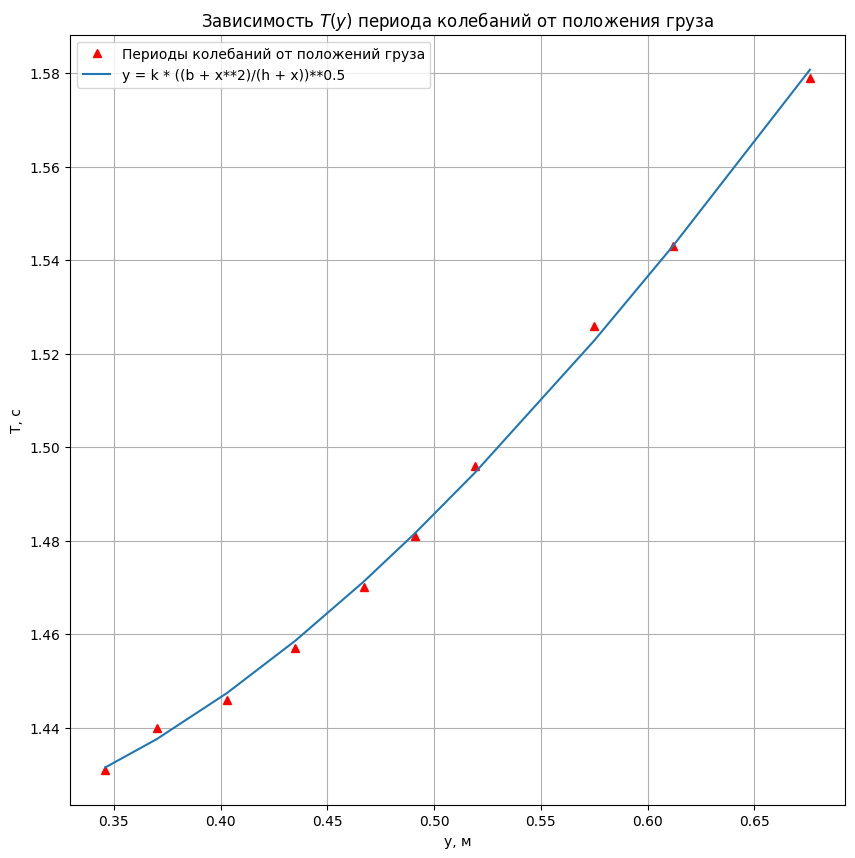
\includegraphics[width=0.8\textwidth]{graphic}
    \caption{Зависимость периода колебаний $T(y)$ от положения ц.м. груза $y$}
\end{figure}

\subsection{Зависимость $u(v)$}

Пусть $u = T^2 x_{\text{ц}}$, а $v = y^2$, тогда пусть $k = \frac{4\pi^2}{g \left( \beta + 1\right)} \approx 0,997$, $b = \frac{4\pi^2}{g \left( \beta + 1\right)} \left( \frac{\beta l^2}{12} + \beta a^2 \right) \approx 0,477$, получаем 
\[u(v) = kx + b \text{ - линейная зависимость}\]

Данные полученные с помощью аппроксимации: $k = 0,997, b = 0,48$ 
\begin{figure}[t]
    \centering
    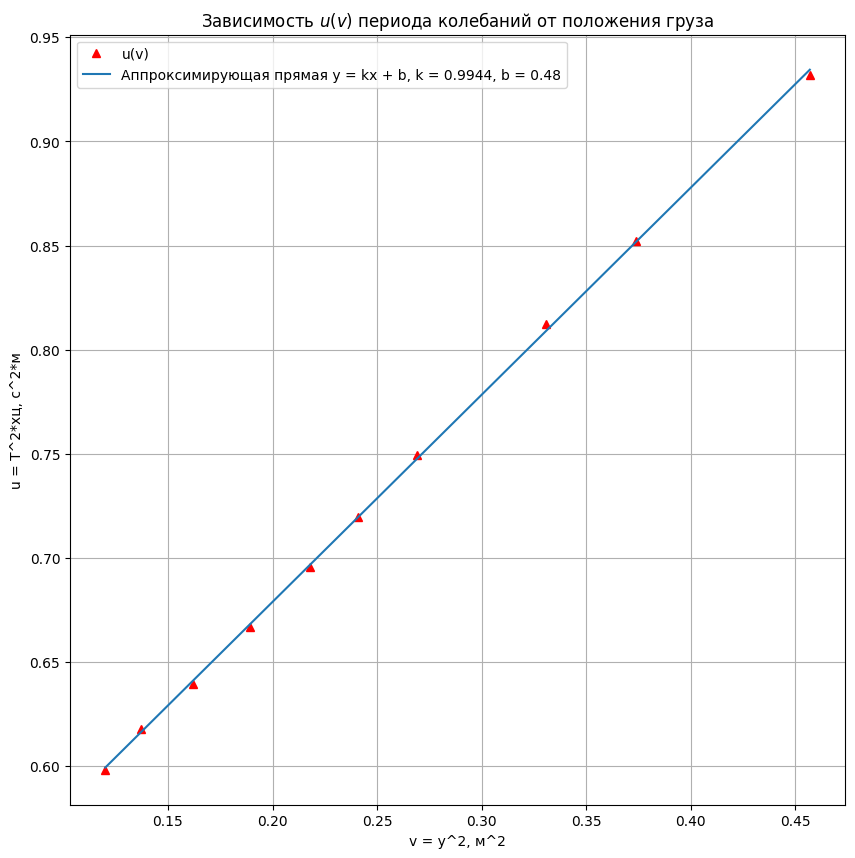
\includegraphics[width=0.8\textwidth]{graphic2}
    \caption{Зависимость $u(v)$}
\end{figure}

Рассчитаем $k$ и $b$ по методу наименьших квадратов:
\[k = \frac{\langle vu \rangle - \langle v \rangle \langle u \rangle}{\langle v^2 \rangle - \langle v \rangle^2} \approx 1,048, b = \langle u \rangle - k \langle v \rangle\ \approx 0,466\]

Отсюда найдем $g$:
\[g = \frac{4\pi^2}{k \left( \beta + 1\right)} \approx 9,854\]

Рассчитаем погрешность $u = T^2 x_{\text{ц}}$ и $v = y^2$:
\[\varepsilon_{u} = \sqrt{\left( 2\frac{\sigma_{T}}{T}\right)^2 + \left( \frac{\sigma_{x_{\text{ц}}}}{x_{\text{ц}}}\right)^2} \approx 0,013\]
\[\varepsilon_{v} = \frac{2\sigma_{y}}{y} \approx 0,0015\]


Рассчитаем случайную погрешность $k$ и $b$:
\[\sigma_{k}^{\text{случ}} = \sqrt{\frac{1}{N-2}\left( \frac{\langle u^2 \rangle - \langle u \rangle^2}{\langle v^2 \rangle - \langle v \rangle^2} - k^2\right)} \approx 0,0003\]
\[\sigma_{b}^{\text{случ}} = \sigma_{k}^{\text{случ}}\sqrt{\langle v^2 \rangle} \approx 8 \cdot 10^5\]

Вычислим систематическую погрешность $k$ и $b$:
\[\sigma_{k}^{\text{сист}} = k\sqrt{(\varepsilon_{v})^2 + (\varepsilon_{u})^2} \approx 0,013\]
\[\sigma_{b}^{\text{сист}} = b\sqrt{(\varepsilon_{v})^2 + (\varepsilon_{u})^2} \approx 0,0063\]

Полная погрешность:
\[\sigma_{k}^{\text{полн}} = k\sqrt{(\varepsilon_{v})^2 + (\varepsilon_{u})^2} \approx 0,013\]
\[\sigma_{b}^{\text{полн}} = b\sqrt{(\varepsilon_{v})^2 + (\varepsilon_{u})^2} \approx 0,0063\]

Тогда $k = 0,997 \pm 0,013 (\varepsilon_{k} = 1,31\%)$ и $b = 0,48 \pm 0,0063 (\varepsilon_{b} = 1,31\%)$.

Тогда:
\[g_{k} = \frac{4\pi^2}{k(\beta + 1)} \approx 9,85\]
\[\sigma_{gk} = g \sqrt{(\varepsilon{k})^2 + (\varepsilon_{\beta})^2} \approx 0,128 (\varepsilon_{gk} = 1,3\%)\]
\[g_{b} = b = \frac{4\pi^2}{g \left( \beta + 1\right)} \left( \frac{\beta l^2}{12} + \beta a^2 \right) \approx 9,85\]
\[\sigma_{gb} = g \sqrt{(\varepsilon{b})^2 + (\varepsilon_{\beta})^2} \approx 0,128 (\varepsilon_{gb} = 1,3\%)\]
Итого:
\[\underline{g_{k} = 9,85 \pm 0,128 \frac{\text{м}}{\text{c}^2} (\varepsilon_{gk} = 1,3\%)}\]
\[\underline{g_{b} = 9,85 \pm 0,128 \frac{\text{м}}{\text{c}^2} (\varepsilon_{gb} = 1,3\%)}\]

\section{Выводы}
В ходе работы мы получили значения ускорения свободного падения 2 способами:
\begin{itemize}
    \item $\underline{g_{k} = 9,85 \pm 0,128 \frac{\text{м}}{\text{c}^2} (\varepsilon_{gk} = 1,3\%)}$
    \item $\underline{g_{b} = 9,85 \pm 0,128 \frac{\text{м}}{\text{c}^2} (\varepsilon_{gb} = 1,3\%)}$
    \item $\underline{g = 9,815 \pm 0,14 \frac{\text{м}}{\text{c}^2} (\varepsilon_{g} = 1,4\%)}$
\end{itemize}

Сравнивая их, получаем что усредненный ответ будет точнее, но при этом в методе МНК меньшее влияние оказывает случайная погрешность. При этом на полную погрешность все равно влияет по большей части систематическая погрешность, а именно неточность измерения экспериментатором центра масс системы и конечное число измерений секундомером времени колебаний.

Полученными данными мы подтвердили теорию для периода колебания физического маятника и подтвердили теорему Гюйгенса экспериментально. 

\end{document}